\chapter{Star Partition and Star Contraction}
\label{ch:graphcon::star}

\begin{preamble}
This chapter covers star partition and star contraction, an
efficient and parallel contraction technique for general graphs. 
\end{preamble}

\section{Star Partition}
\label{sec:graphcon::star::partition}

\begin{gram}
In an edge partition, if an edge incident on a vertex~$v$ is selected
as a block, then none of the other edges incident on $v$ can be their
own block (\chref{graphcon::edge}). 
%
This limits the effectiveness of the edge partition technique, because
it is unable to contract graphs with high-degree vertices
significantly.
%
In this section, we describe an alternative technique: star partition.
\end{gram}

\begin{group}
\begin{definition}[Star Partition]
A~\defn{star partition} of a graph $G$ is a partition where each block
is a vertex-induced subgraph of $G$ with respect to a star.
\end{definition}

\begin{example}
\label{ex:graphcon::star-partition}
Consider star graph with center $v$ and eight satellites.
  \begin{center}
  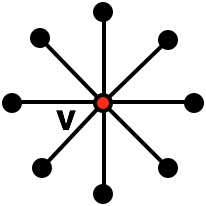
\includegraphics[width=1.5in]{./media-star/star-graph1.jpg}
  \end{center}

\begin{itemize}
\item A partition consisting of the whole graph is a star partition, where 
the only block is the graph itself, induced by the star graph.

\item A partition where each block is an isolated vertex is a star
  partition, because each block is a vertex-induced subgraph of a
  single vertex, which is a star.
\end{itemize}

\end{example}


\begin{example}
\label{ex:graphcon::star-partition-2}

Consider the graph shown below on the left.
%
To partition this graph, we first find two disjoint stars, which are
highlighted.
%
Each star induces a block consisting of its vertices and the
corresponding edges of the graph.
%
These two blocks form a star partition the graph.
%
%% TODO: Comment this out in favor of the important block below.
Note that in a star partition, a partition might not be a star.
\begin{center}
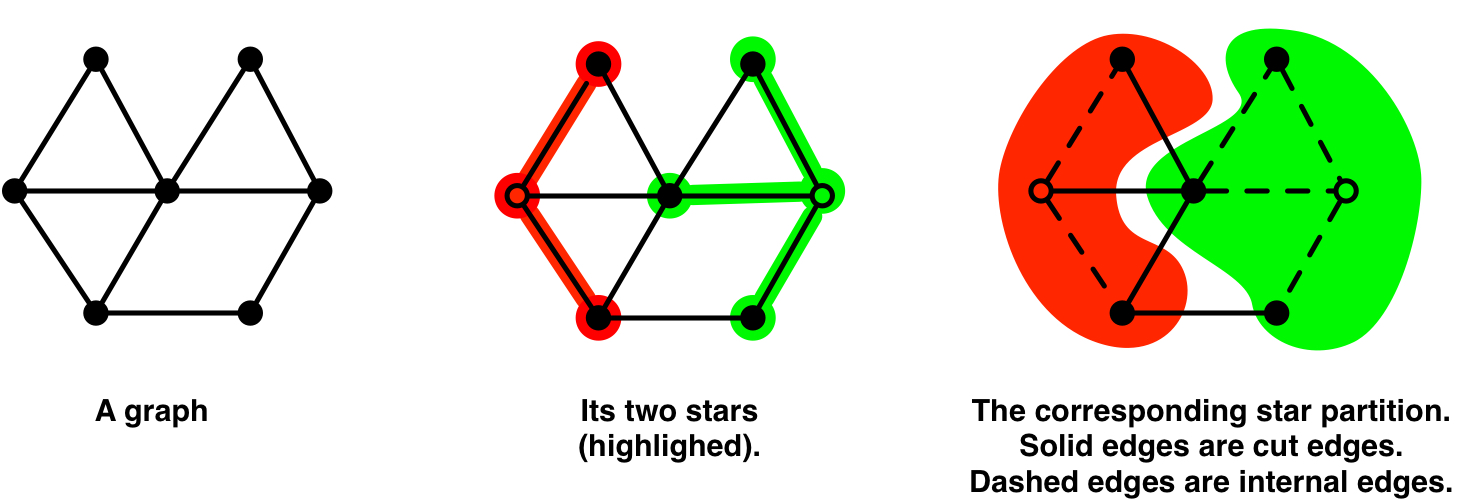
\includegraphics[width=0.9\textwidth]{./media-star/star-decomposition-1.jpg}
\end{center}
\end{example}
\end{group}

%% \begin{important}
%% In a star partition, a partition might not be a star.
%% \end{important}
%% \begin{teachask}
%% How can we star-partition a graph? 
%% \end{teachask} 

\begin{gram}[Sequential Construction of a Star Partition]
We can construct a star partition sequentially by iteratively adding
stars until the vertices are exhausted as follows.

\begin{itemize}

\item Select an arbitrary vertex $v$ from the graph and make $v$ the
  center of a star.

\item Attach as satellites all the neighbors of $v$ in the graph.

\item Remove $v$ and its satellites from the graph.

\end{itemize}
%
\end{gram}

\begin{group}
\begin{gram}[Parallel Star Partition]
%% \begin{teachask}
%% How can we star partition a graph in parallel? 
%% \end{teachask} 
%
We can construct a star partition in parallel by making local
independent decisions for each vertex, and using randomization to
break symmetry.
%
%% \begin{teachask}
%% Can you think of a randomized approach for selecting stars?
%% \end{teachask}
%
One approach proceeds as follows. 
%
\begin{itemize}
\item Flip a coin for each vertex.

\item If a vertex flips heads, then it becomes the center of a star. 

%% \item If a vertex flips tails, then it attempts to become a satellite
%%   by finding a neighbor that has flipped heads.  If no such neighbor
%%   exists (all neighbors have flipped tails or the vertex is isolated),
%%   then the vertex becomes a center.
%%%% TODO: The following seems to be a better explanation
\item If a vertex flips tails, then there are two cases.
\begin{itemize}
\item The vertex is isolated (it has no neighbors).  In this case, it
  becomes a center.
\item The vertex has a neighbor.  In this case, the vertex looks for a
  neighbor that flipped heads.  If there is such a neighbor, then it
  chooses one arbitrarily, and becomes a satellite for that
  neighbor. Otherwise, all neighbors have flipped tails and the
  vertex becomes a center.
\end{itemize}
\end{itemize}

%
%% \begin{teachask}
%% Is this algorithm guaranteed to create the smallest number of stars?
%% \end{teachask}
%
This approach is not optimal in the sense that it might not always
create the smallest number of stars.
%
As we shall see, such suboptimality is acceptable, because we only
need to reduce the size of the graph by a constant factor.
\end{gram}

\begin{example}[Randomized Star Partition]
\label{ex:startpartition}
An example star partition. Vertices $\vname{a}$ and $\vname{b}$, which
flip heads, become centers. Vertices $\vname{c}$ and $\vname{e}$,
which flipped tails, attempt to become satellites by finding a center
among their neighbors, breaking ties arbitrarily.
%
If a vertex does not have a neighbor that is a center (flipped heads),
then it becomes a singleton star (e.g., vertex $d$).
%

The resulting star partition has three stars: the star with center $\vname{a}$ (with no
satellites), the star with center $\vname{b}$ (with two satellites),
and the singleton star $\vname{d}$.
%
The star partition thus yields three blocks, which are defined by the
subgraphs induced by each star.

\begin{center}
  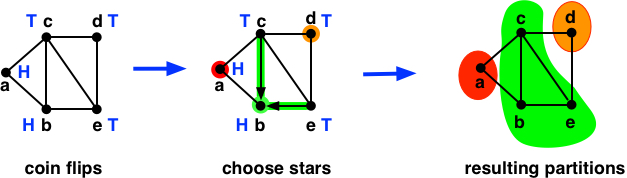
\includegraphics[width=6in]{./media-star/star-find0.jpg}
\end{center}

\end{example}
\end{group}


\begin{group}
%require an undirected graph $G=(V,E)$ and round number $i$
%return $V'$ = remaining vertices after contraction,
%          $P$ = mapping from $V$ to $V'$
\begin{algorithm}[Parallel Star Partition]
\label{alg:graphcon::starPartition}

To specify the star-partition algorithm, we need
a source of randomness.
%
We assume that each vertex is given a (potentially infinite) sequence
of random and independent coin flips. The $i^{th}$ element of the
sequence can be accessed via the function
\[
\cheads(v,i) : V \times \mathbb{Z} \to \mathbb{B}, 
\]
which returns $\cd{true}$ if the $i^{th}$ flip on vertex $v$ is heads
and false otherwise. 

\[
\begin{array}{ll}
1 & \cdvar{starPartition}~(G=(V,E),i) =
\\
2 & ~~~~\cd{let}
\\
3 & ~~~~~~~~\cd{(* Find the arcs from satellites to centers. *)}
\\
4 & ~~~~~~~~\mathit{TH} = \csetf{(u,v) \in E}{\neg \cheads(u,i) \land \cheads(v,i)} %@\label{line:flip}\vspace{.1in}@
\\
5 & ~~~~~~~~\cd{(* Partition map: satellites map to centers *)}
\\
6 & ~~~~~~~~P_s = \bigcup_{(u,v) \in \mathit{TH}} \cset{u \mapsto v}
% \label{line:starmerge}
\\
7 & ~~~~~~~~\cd{(* Centers are non-satellite vertices *)}
\\
8 & ~~~~~~~~V_c = V \setminus \cdvar{domain}(P_s)
\\
9 & ~~~~~~~~\cd{(* Map centers to themselves *)}
\\
10 & ~~~~~~~~~P_c = \cset{u \mapsto u : u \in V_c} % \label{line:self}
\\
11 & ~~~~\cd{in}
\\
12 & ~~~~~~~~(V_c, P_s \cup P_c)
\\
13 & ~~~~\cd{end}
\end{array}
\]

The function $\cdvar{starPartition}$ takes as argument a graph and a round
number, and returns a graph partition specified by a set of centers and
a partition map from all vertices to centers.
%
The algorithm starts by flipping a coin for each vertex and selecting
the edges that point from tails to heads---this gives the set of edges
$\mathit{TH}$.
%
In this set of edges, there can be multiple edges from the same
non-center. Since we want to choose one center for each satellite, we
we remove duplicates in Line \linegcstarmerge{}, by creating a set of
singleton tables and merging them, which selects one center per
satellite.
%
This completes the selection of satellites and their centers. 
%

Next, the algorithm determines the set of centers as all the
non-satellite vertices.
%
To complete the process, the algorithm maps each center to itself
(Line~\linegcstarself{}).
%
These operations effectively promote unmatched non-centers to centers,
forming singleton stars, and matches all centers with themselves.
%
Finally, the algorithm constructs the partition map by unite the
mapping for the satellites and the centers.
%
Recall that the partition map is a mapping from each vertex to the
representative vertex of its partition, which in this case is the
center.
\end{algorithm}

\begin{note}
Since most machines don't have true sources of randomness, in practice
the function $\cdvar{heads}$ is usually implemented with a
pseudorandom number generator or with a good hash function.

In the algorithm, Line~\linegcstarmerge{} creates a set of
singleton tables and merging them.
%
This can be implemented using sets and tables as follows.
%
\[
\begin{array}{ll}
  \cdvar{Set.reduce}
  & (\cdvar{Table.union}~(\cfn{(x,y)}{x}))
\\
& \emptyset
\\
& \cset{\cset{u \mapsto v} : (u,v) \in \mathit{TH}}
\end{array}
\]
Note that we supply to the $\cdvar{union}$ operation a function that selects the first of the two possibilities; this is an arbitrary choice and we could have favored the second.

\end{note}

\begin{example}
Consider the star partition illustrated below.
\begin{center}
  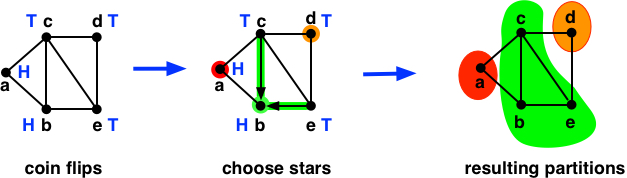
\includegraphics[width=6in]{./media-star/star-find0.jpg}
\end{center}

The  star-partition algorithm proceeds on this example as follows.
%
First, it computes
%
\[
\mathit{TH} =
\cset{(\vname{c},\vname{a}),(\vname{c},\vname{b}),(\vname{e},\vname{b})},
\]
%
as the edges from satellites to centers.  
%
Now, it
converts each edge into a singleton table, and merges all the tables
into one
table, which is going to become a part of the partition map:
%
\[
P_s = \cset{\vname{c} \mapsto \vname{b},\vname{e} \mapsto \vname{b}}.
\]
%
Note that the edge $(\vname{c},\vname{a})$ has been removed since when
uniting the tables, we select only one element for each key in the
domain.  
%
Now for all remaining vertices
%
$V' = V \setminus \cdvar{domain}(P) = \cset{\vname{a},\vname{b},\vname{d}}$
we map them to themselves, giving:
%
\[
P_c = \cset{\vname{a} \mapsto \vname{a}, \vname{b} \mapsto \vname{b},
  \vname{d} \mapsto \vname{d}}.
\]
%
The vertices in $P'$ are the centers.
%
Finally we merge $P$ and $P'$ to obtain the partition map
%
\[
P_s \cup P_c = \cset{\vname{a} \mapsto \vname{a}, \vname{b} \mapsto \vname{b}, \vname{c} \mapsto \vname{b}, \vname{d} \mapsto
    \vname{d}, \vname{e} \mapsto \vname{b}}.
\]
\end{example}
\end{group}

%\end{section}

%% \begin{todo}
%% This theorem needs a proof.  What is the graph representation? 
%% It seems like it is an edge set representation.

%% The big union would require logn span do we need inject here?

%% \end{todo}


